\documentclass{sig-alternate}

\begin{document}

\title{Seguimiento de un blanco m\'{o}vil}

\numberofauthors{2}

\author{
    \alignauthor
    Villa Fern\'{a}ndez, Santiago\\
    \email{svillafe@alu.itba.edu.ar} \\
    \ \\
    Gomez Vidal, Maximiliano\\
    \email{dgomezvi@alu.itba.edu.ar} \\
    \alignauthor
    Sessa, Carlos\\
    \email{csessa@alu.itba.edu.ar} \\
    \ \\
    Abramowicz, Pablo\\
    \email{pabramow@alu.itba.edu.ar} \\
}

\maketitle

\begin{abstract}
En este art\'{i}culo se modela un sistema de seguimiento de blancos a lazo 
cerrado. Se analiza el comportamiento del sistema con distintos controladores
de tipo proporcional, integral y derivativo.
\end{abstract}

\keywords{Seguimiento de blancos, sistema de control, controlador proporcional,
controlador derivativo, controlador integral}

\section{Introducci\'{o}n}\label{introduccion}
Un sistema de seguimiento de blancos consiste en un radar y una antena.
Se desea que la antena apunte al blanco, por lo que se debe ajustar su 
posici\'{o}n  seg\'{u}n corresponda. Para esto se incluye un controlador que 
compara el \'{a}ngulo de la antena con el \'{a}ngulo en donde se encuentra el 
objetivo y proporciona el torque correspondiente para minimizar la discrepancia 
entre ambos.

En la secci\'{o}n \ref{modelo} se describe el modelo del sistema. En la
secci\'{o}n \ref{simulaciones} se realizan las simulaciones correspondientes
a los tres tipos de controladores utilizados: proporcional, integral y 
derivativo. Por \'{u}ltimo, se exponen las conclusiones en la secci\'{o}n
\ref{conclusiones}.

\section{Modelo}\label{modelo}
La din\'{a}mica de la antena se modela seg\'{u}n la ecuaci\'{o}n diferencial:
\begin{equation}
\label{dinamica_antena}
I \ddot\theta = - b \dot\theta + u(t)
\end{equation}
donde $\theta$ es el \'{a}ngulo que corresponde a la direcci\'{o}n en la que
apunta el radar, $I$ es el momento de inercia de la antena y $b$ es una 
constante positiva que vincula la fuerza viscosa que act\'{u}a sobre la antena.
El torque que producen los motores sobre la antena est\'{a} representado por 
la funci\'{o}n $u$.

Se desea que el sistema sea a lazo cerrado. Para esto se mide el \'{a}ngulo
$\theta$ de la antena y se lo compara con el \'{a}ngulo $\theta_{R}$ que denota
la ubicaci\'{o}n real del objetivo. La diferencia entre ambos constituye una
se\~{n}al de error $e(t) = \theta_{R}(t) - \theta(t)$ que se ingresa nuevamente 
al controlador.

\section{Simulaciones}\label{simulaciones}
Para realizar la simulaci\'{o}n se consideran los par\'{a}metros 
$I = 0.004\ kg\ m^{2}$ y $b = 0.02\ kg\  m^{2}\ s^{-1}$. Tambi\'{e}n se establece
que el blanco se mueve de acuerdo a $\theta_{R}(t) = 0.01 t$.
Se estudian tres tipos de controladores: proporcional, integral y derivativo.
En todos los casos se utiliza el m\'{e}todo de Runge-Kutta de orden $4$ para
la resoluci\'{o}n num\'{e}rica de las ecuaciones diferenciales.

\subsection{Controlador proporcional}\label{proporcional}
Se propone un primer controlador que se comporta seg\'{u}n la 
ecuaci\'{o}n lineal:

\begin{equation}
\label{error_modelo}
u(t) = K e(t)
\end{equation}

donde $e(t)$ es la se\~{n}al de error. La relaci\'{o}n de entrada-salida 
puede expresarse entonces como la siguiente ecuaci\'{o}n diferencial:

\begin{equation}
\label{ecuacion_modelo1}
I \ddot\theta = - b \dot\theta + K(\theta_R(t) - \theta(t))
\end{equation}

La descripci\'on en variables de estado resulta:

\begin{equation}
\label{var_estados_model1}
\begin{cases} 
    \dot x_1 = x_2 \\
    \dot x_2 = -\frac{b}{I} x_2 + \frac{K}{I} (\theta_R(t) - x_1)
\end{cases}
\end{equation}

donde $x_1 = \theta$, $x_2 = \dot \theta$ y la salida es $\theta=x_1$.

Siendo la estabilidad del sistema dependiente de la excitaci\'{o}n $u(t)$,
es posible estudiar la estabilidad utilizando el polinomio caracter\'istico. 
Si la parte real de las ra\'{i}ces de
todos los autovalores del polinomio caracter\'istico es negativa, entonces 
el sistema es estable. Entonces, presentando la ecuaci\'{o}n $4$ en forma vectorial:
\begin{center}
$
\dot x(t) = 
\left( \begin{array}{cc}
0 & 1 \\
-\frac{K}{I} & -\frac{b}{I}
\end{array} \right)
\left( \begin{array}{c}
x_1 \\
x_2
\end{array} \right)
= Ax(t)
$
\end{center}
El polinomio caracter\'istico de $A$ es:

\begin{equation}
 P( \lambda ) = |A - \lambda I|
\end{equation}

Aplic\'{a}ndolo a la matriz que hemos definido resulta:

\begin{equation}
 P( \lambda ) = |A - \lambda I| = 
\left| \begin{array}{cc}
-\lambda & 1 \\
-\frac{K}{I} & -\frac{b}{I}-\lambda
\end{array} \right| 
=
\lambda^2 + \frac{b}{I} \lambda + \frac{K}{I}
\end{equation}

Siendo los autovalores las ra\'ices de $P(\lambda) = 0$, las mismas son:

\begin{equation}
 \lambda{1,2} = - \frac{b}{2I} \pm \frac{1}{2} \sqrt{\frac{b^2}{I^2}-4\frac{K}{I}}
\end{equation}

Se observa que para todo $K > 0$ las raices son negativas, por lo que el sistema 
es estable para $K \in (0,+\infty)$.\\
Respecto a la presencia de oscilaciones en r\'{e}gimen estacionario, uno de los 
autovalores (ecuaci\'on $6$) debe tener parte imaginaria no nula y en 
consecuencia el determinante debe ser negativo. Esta condici\'on se asegura 
para valores de $K > \frac{b^2}{4I}$. 

En la figura $1$ se observan las distintas salidas al ir variando los valores
de la constante $K$. En la figura $4$ se muestra el error relativo porcentual,
definido por:
\begin{equation}
\label{ecuacion_error_relativo_porcentual}
E\%(t)=\frac{\theta_{R}(t) - \theta(t)}{\theta_{R}(t)}
\end{equation}
Se observan oscilaciones que se estabilizan alrededor de los cinco segundos.

\subsection{Controlador integral}\label{integral}
Otro tipo de controlador es el integral, cuya forma es:

\begin{equation}
\label{error_modelo2}
u(t) = K_i \int_0^t e(\tau) d\tau
\end{equation}

siendo $e(t)$ la se\~nal de error. Se obtiene la relaci\'{o}n de
entrada-salida como:

\begin{equation}
\label{ecuacion_modelo2a}
I \ddot\theta = - b \dot\theta + K_i \int_0^t \theta_R(\tau) - \theta(\tau) d\tau
\end{equation}

La descripci\'{o}n en variables de estado de la ecuaci\'on $10$ resulta:

\begin{equation}
\label{var_estados_model2}
\begin{cases} 
    \dot x_1 = x_2 \\
    \dot x_2 = x_3 \\
    \dot x_3 = -\frac{b}{I} x_3 - \frac{K_i}{I} \left[ \int_0^t \theta_R(\tau) d\tau -x_1 \right]
\end{cases}
\end{equation}

donde $x_1 = \int_0^t \theta(\tau) d\tau$, $x_2 = \theta$, $x_3 = \dot \theta$ 
y la salida es $\theta=x_2$.\\
Representando dichas variables en forma matricial:

\begin{center}
$
\dot x(t) = 
\left( \begin{array}{ccc}
0 & 1 & 0\\
0 & 0 & 1\\
-\frac{K_i}{I} & 0 & -\frac{b}{I}
\end{array} \right)
\left( \begin{array}{c}
x_1 \\
x_2 \\
x_3
\end{array} \right)
= Ax(t)
$
\end{center}

El polinomio caracter\'istico queda definido como:

\begin{equation}
 P( \lambda ) = |A - \lambda I| = 
\left| \begin{array}{ccc}
-\lambda & 1 & 0\\
\\ 0 & -\lambda & 1 \\
-\frac{K_i}{I} & 0 & -\frac{b}{I}-\lambda
\end{array} \right| 
=
\lambda^3 + \frac{b}{i}\lambda^2 + \frac{K_i}{I}
\end{equation}

Se concluye que para este polinomio caracter\'istico 
siempre existe alguna ra\'iz positiva para $K_i \in (0,+\infty)$. Por lo tanto, 
el sistema no es estable, presentando oscilaciones cuya amplitud aumenta
en el tiempo. Este fen\'{o}meno se observa claramente en la figura $2$.
El error relativo porcentual se muestra en la figura $5$, presentando tambi\'{e}n
las oscilaciones caracter\'{i}sticas.

\subsection{Controlador derivativo}\label{derivativo}
Como tercer controlador se propone un modelo derivativo, cuyo comportamiento
se define como:

\begin{equation}
\label{error_modelo3}
u(t) = K_d \frac{d e(t)}{d t}
\end{equation}

siendo $e(t)$ la se\~{n}al de error. Se obtiene la relaci\'{o}n de entrada-salida 
como:

\begin{equation}
\label{ecuacion_modelo2b}
I \ddot\theta = - b \dot\theta + K_d (\dot\theta_R(t) - \dot\theta(t))
\end{equation}

Se representa la ecuaci\'on $14$ en variables de estado como:

\begin{equation}
\label{var_estados_model3}
\begin{cases} 
    \dot x_1 = x_2 \\
    \dot x_2 = \frac{K_d}{I} \dot\theta_R(t) - x_2 \frac{b+ K_d}{I}
\end{cases}
\end{equation}

donde $x_1 = \theta$, $x_2 = \dot \theta$ y la salida es $\theta=x_1$.\\
Representando dichas variables en forma matricial resulta:

\begin{center}
$
\dot x(t) = 
\left( \begin{array}{ccc}
0 & 1 \\
0 & -\frac{b+K_d}{I}
\end{array} \right)
\left( \begin{array}{c}
x_1 \\
x_2
\end{array} \right)
= Ax(t)
$
\end{center}

El polinomio caracter\'istico queda definido como:

\begin{equation}
 P( \lambda ) = |A - \lambda I| = 
\left| \begin{array}{cc}
- \lambda & 1 \\
0 & - \lambda - \frac{b+K_d}{I}
\end{array} \right| 
=
\lambda^2 + \lambda \frac{b+K_d}{I}
\end{equation}

Las ra\'{i}ces de este polinomio son $0$ y $-\frac{b+K_d}{I}$, por lo que el
sistema es estable siempre y cuando $K_d \in (-b, +\infty)$.

En la figura $3$ se presenta la salida para distintos valores de $K_d$. En la
figura $6$ se muestra el error relativo porcentual para este tipo de controlador.

\section{Conclusiones}\label{conclusiones}
A partir de las simulaciones se observa que el controlador proporcional es el
m\'{a}s estable y preciso de los tres controladores analizados. El
controlador integral resulta sumamente inestable, presentando oscilaciones
que aumentan su amplitud con el paso del tiempo. Para determinados casos puede
utilizarse un controlador derivativo, aunque depender\'{a} de los par\'{a}metros
del radar, pues resulta menos efectivo que el proporcional.

\begin{figure*}[hp]
\label{mProporcional}
\centering
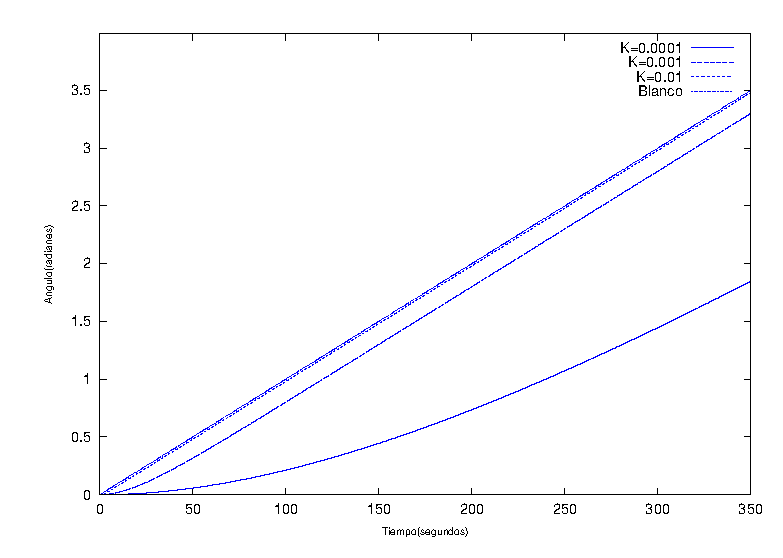
\includegraphics[scale=0.8]{graficos/mProporcional}
\caption{Salida $\theta(t)$ con controlador proporcional}
\end{figure*}

\begin{figure*}[hp]
\label{mIntegral}
\centering
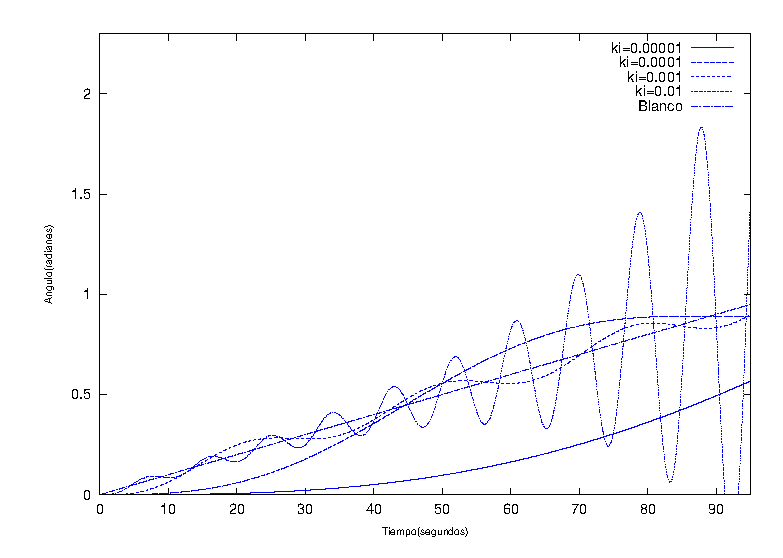
\includegraphics[scale=0.8]{graficos/mIntegral}
\caption{Salida $\theta(t)$ con controlador integral}
\end{figure*}

\begin{figure*}[hp]
\label{mDerivativo}
\centering
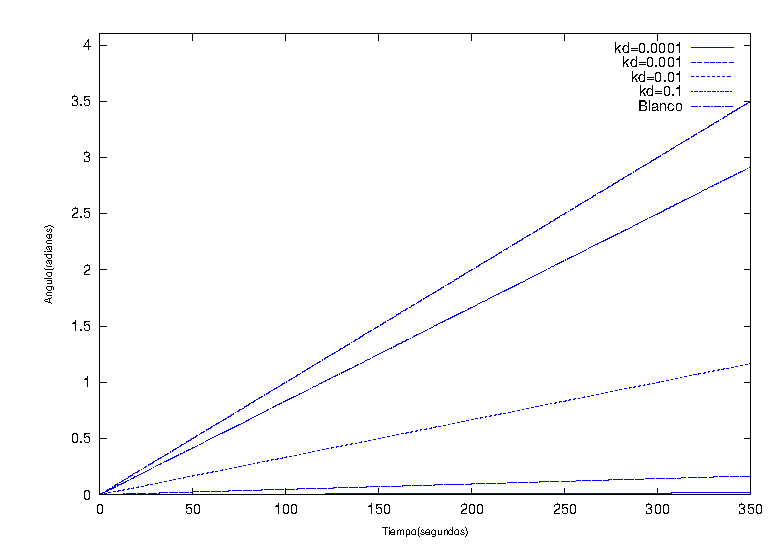
\includegraphics[scale=0.8]{graficos/mDerivativo}
\caption{Salida $\theta(t)$ con controlador derivativo}
\end{figure*}

\begin{figure*}[hp]
\label{errorPorcentualMProporcional}
\centering
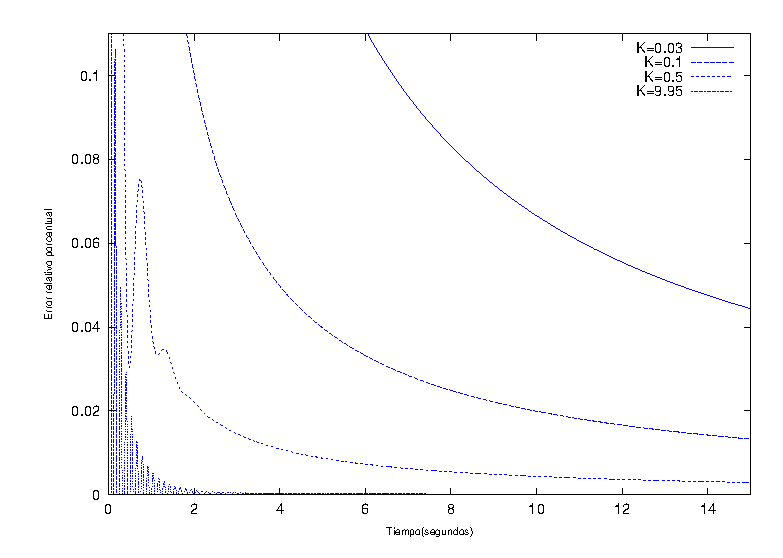
\includegraphics[scale=0.8]{graficos/errorPorcentualMProporcional}
\caption{Error relativo porcentual al utilizar un controlador proporcional}
\end{figure*}

\begin{figure*}[hp]
\label{errorMIntegral}
\centering
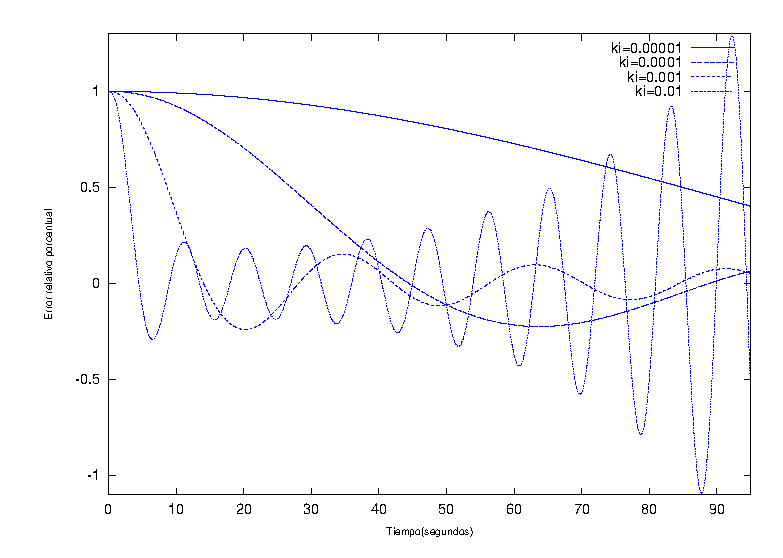
\includegraphics[scale=0.8]{graficos/errorMIntegral}
\caption{Error relativo porcentual al utilizar un controlador integral}
\end{figure*}

\begin{figure*}[hp]
\label{errorPorcentualMDerivativo}
\centering
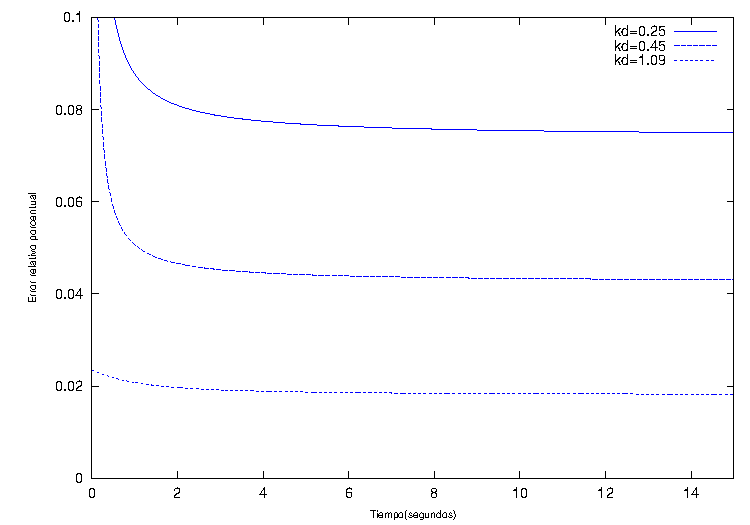
\includegraphics[scale=0.8]{graficos/errorPorcentualMDerivativo}
\caption{Error relativo porcentual al utilizar un controlador derivativo}
\end{figure*}
\end{document}
